\section{Greedy Algorithm Based on Huffman coding}

\subsection{Description}


% \begin{algorithm}[H]
% 	\caption{Brute force algorithm} 
% 	\begin{algorithmic}[1]
%     \State initialize empty array $trees$
% 	\Procedure{BF}{nodes}
% 	    \If{$nodes$ contain only one node}
% 	        \State append $nodes$ to $trees$
% 	        \State \Return
% 	    \EndIf
% 	    \State $pairs \gets \{(nodes[i], nodes[j]): i < j\}$
%         \For{every $(i,j) \in pairs$}
%         		\If{$i$ and $j$ can merge}
%         		    \State $newNodes \gets$ merge $i$ and $j$
%         		    \State \Call{BF}{$newNodes$}
%                 \EndIf
%         \EndFor
%     \EndProcedure
% 	\State read $p(x)$ and initialize corresponding $nodes$
% 	\State \Call{BF}{$nodes$}
% 	\State find the tree with minimum expected length in $trees$
% 	\end{algorithmic} 
	
% \end{algorithm}

The most straightforward algorithm is search by brute force. This algorithm is promised to find the precise result but is too slow for large-scale problems. Therefore, we try to use the same method of Huffman coding. In every iteration we still try to merge the two nodes with minimum sum of probabilities, if possible. This gives us the prototype of a greedy algorithm based on Huffman coding.

\begin{algorithm}
	\caption{Greedy algorithm based on Huffman coding} 
	\begin{algorithmic}[1]
	\Procedure{GreedyHuffman}{nodes}
	    \If{$nodes$ contains only one node}
	        \State \Return $nodes$
	    \EndIf
	    \State $pairs \gets \{(nodes[i], nodes[j]): i < j\}$
	    \State sort $pairs$ by the sum of probabilities in ascending order
        \For{every $(i,j) \in pairs$}
        		\If{$i$ and $j$ can merge}
        		    \State $newNodes \gets$ merge $i$ and $j$
        		    \State $tree \gets$ \Call{GreedyHuffman}{$newNodes$}
        		    \If{$tree \ne \emptyset$}
        		        \State \Return $tree$
        		    \EndIf
                \EndIf
        \EndFor
        \State \Return $\emptyset$
    \EndProcedure
	\State read $p(x)$ and initialize corresponding $nodes$
	\State $tree \gets$ \Call{GreedyHuffman}{$nodes$}
	\end{algorithmic} 
	
\end{algorithm}

The critical part of the algorithm is how we judge whether two nodes can be merged (line 8). The following proposition describes this process mathematically, but it is not practical in practice. The algorithm of the process needs to be designed specifically to get a better performance.

\begin{definition}
The set of possible values of $X$ at a certain node of a decision tree is called the candidates of the node.
\end{definition}

\begin{proposition}
Assume that $A$ and $B$ are the candidates of two nodes. Then the two nodes can be merged if and only if $\exists C \in \mathscr{A}$, $(A \cup B)\setminus C \in \{A, B\}$.
\end{proposition}

\subsection{First Try to Solving the DNA Detection Problem}

The following proposition instructs us how to judge whether two nodes can be merged for this problem.

\begin{proposition}
Assume that $A$ and $B$ are the candidates of two nodes. Then the two nodes can be merged if and only if any of the two conditions holds:
    \begin{enumerate}[label=(\arabic*)]
        \item $A$ or $B$ is continuous.
        \item $\min A > \max B$ or $\min B > \max A$.
    \end{enumerate}
\end{proposition}

Using these two conditions, we implemented our first algorithm that deals with the DNA detection problem. We carried out a experiment by generating \num{10000} random $p(x)$ with $n=6$ and compare the result of the brute force algorithm and the Huffman-based algorithm. The results of the experiment indicate that the result of this algorithm is rather close to the optimal value. The result of each data is represented by a point in Figure \ref{fig:greedy_huffman_1}. The red line in Figure \ref{fig:greedy_huffman_1} is the optimal bound, because the brute force algorithm is promised to find the precise optimal value. We can see that most of the points are close to the red line, and many of them exactly lie on the red line, which means they reach the optimal bound. In fact, around $60\%$ of the data reach the optimal bound.

This intuition is further confirmed by Figure \ref{fig:greedy_huffman_2}. Let $L_b$ and $L_g$ be the expected length of the brute force algorithm and the Huffman-based algorithm, respectively. We define that $\text{gap} = \frac{L_g-L_b}{L_b}$. Although the maximum of gap is around $35\%$, in most cases, the gap is less than $10\%$. Therefore, the result of the Huffman-based algorithm is very satisfactory.

\begin{figure}[H]
    
    \centering
    
    \begin{subfigure}{0.45\textwidth}
        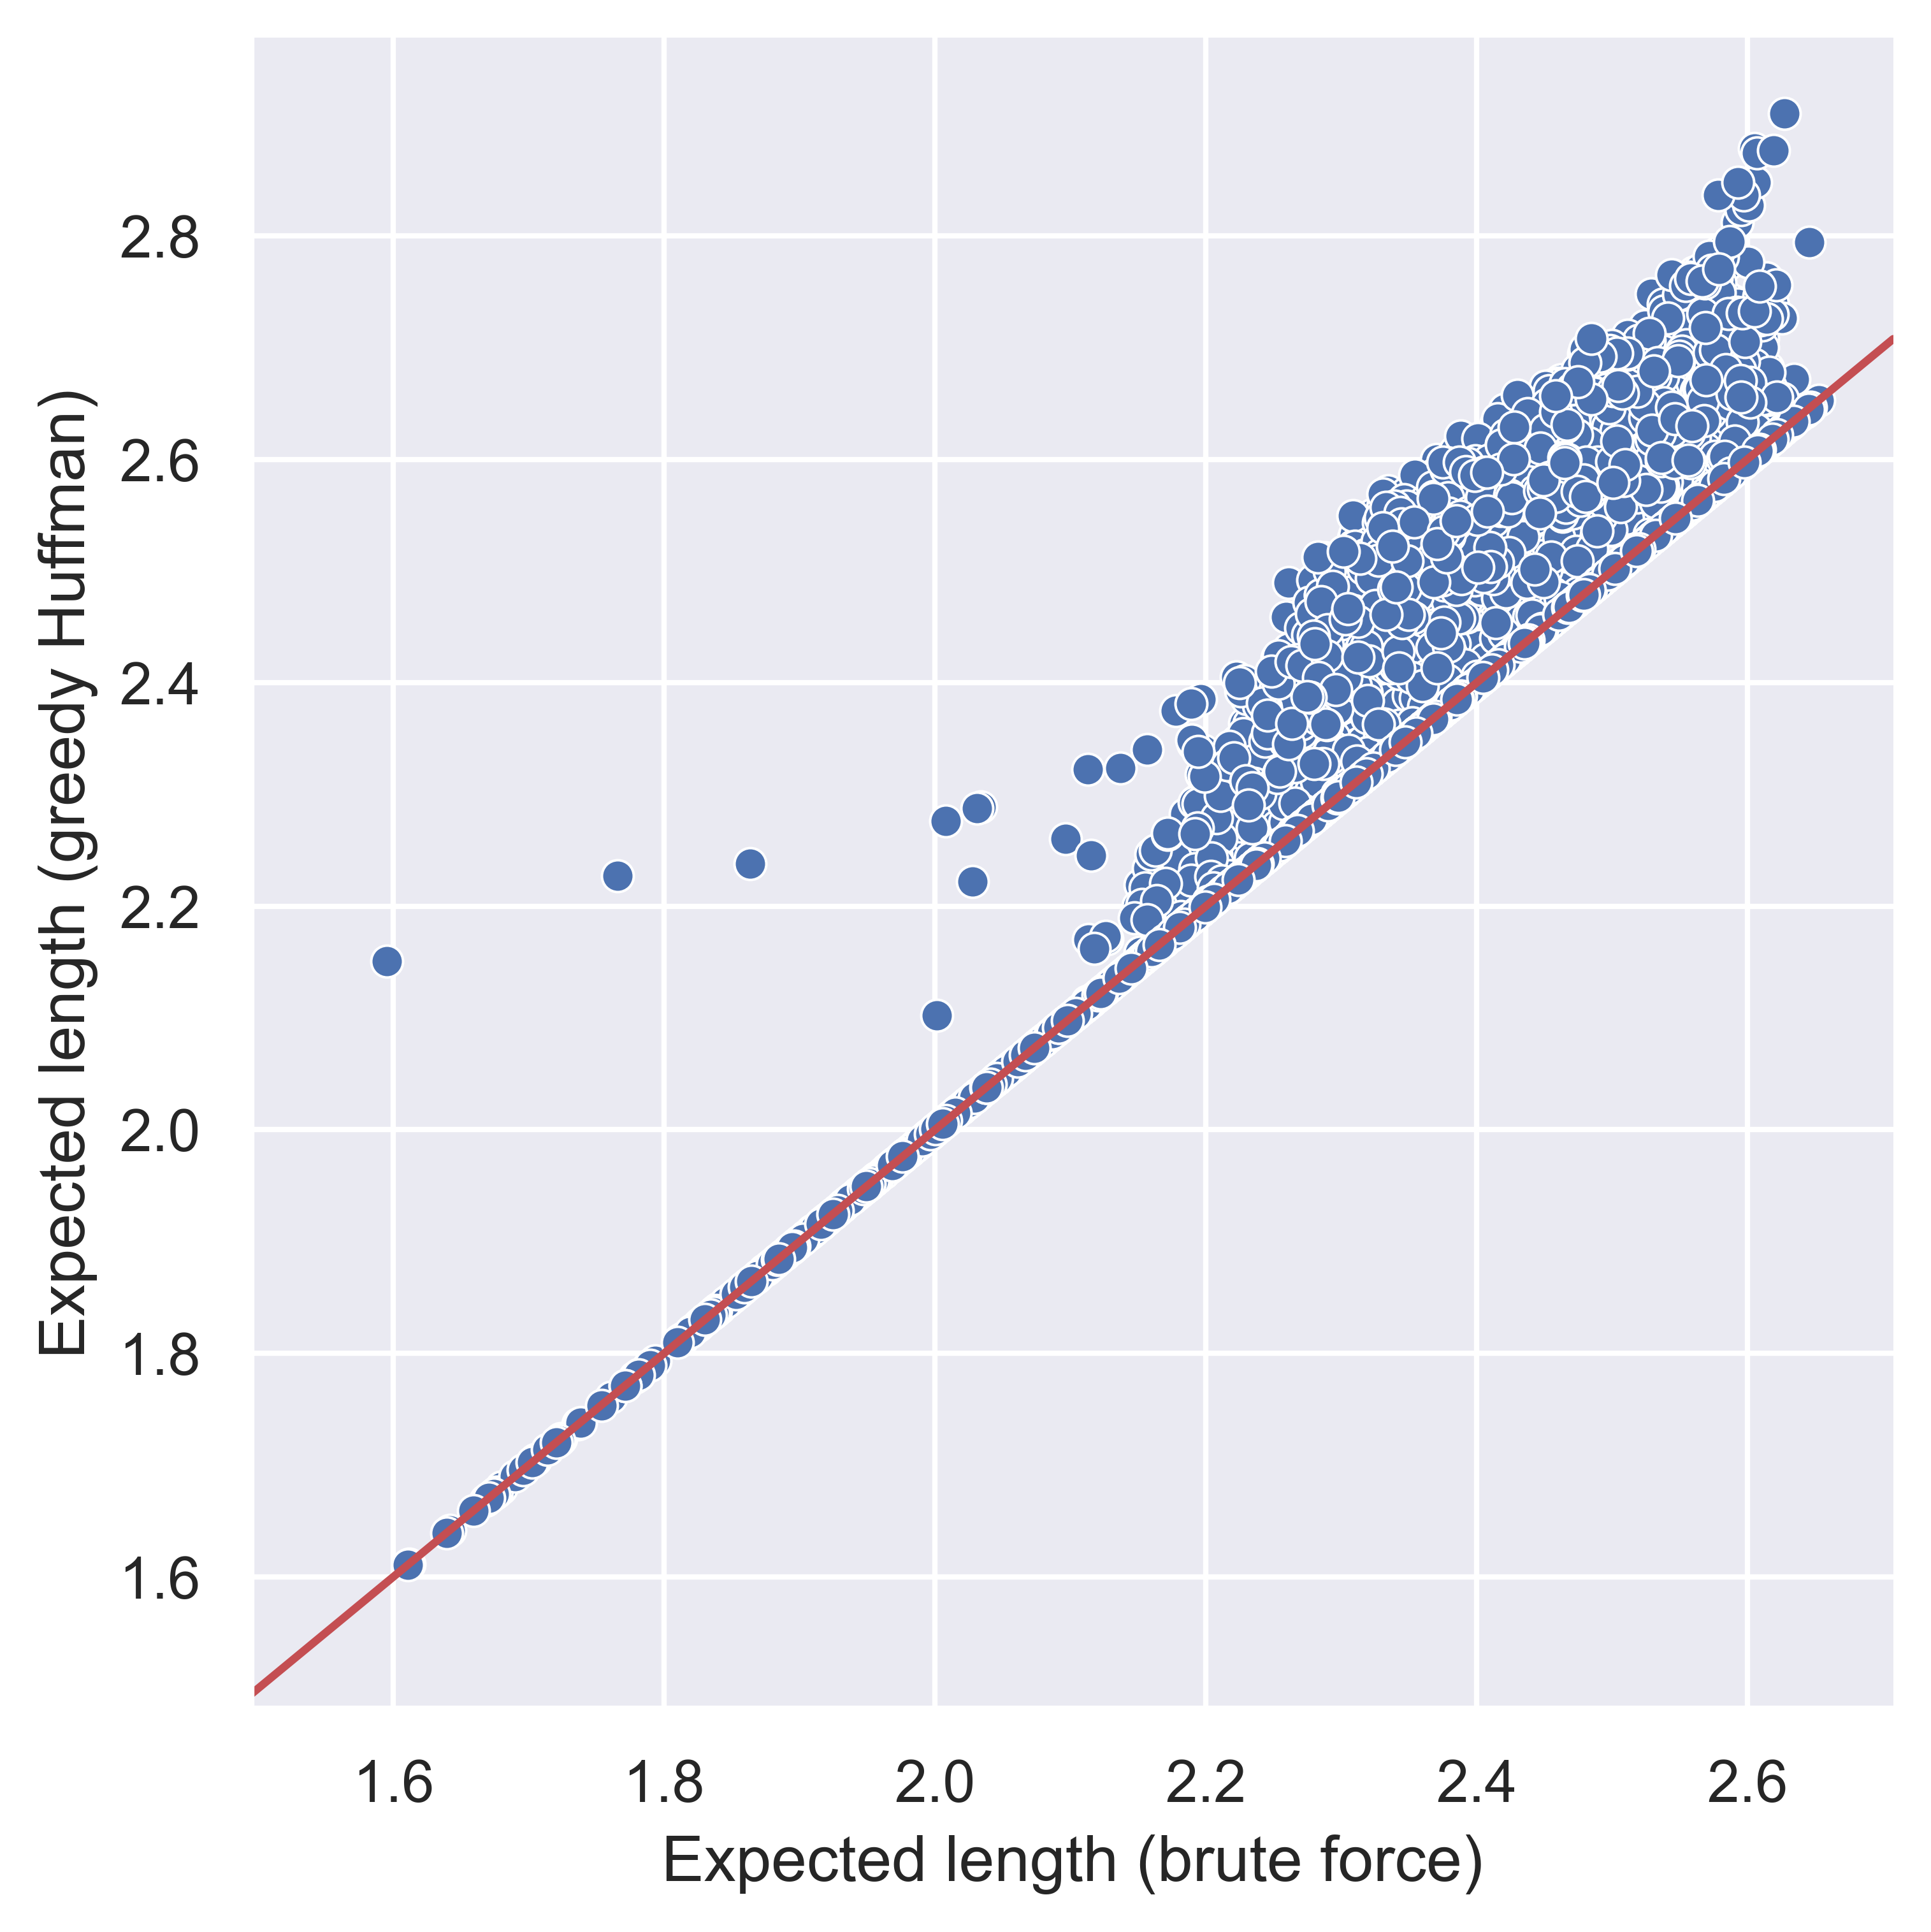
\includegraphics[width=1.0\textwidth]{figure/greedy_huffman_fig1.png}
        \caption{Expected lengths of the brute force algorithm and the Huffman-based algorithm.}
    \label{fig:greedy_huffman_1}
    \end{subfigure}
    \begin{subfigure}{0.45\textwidth}
    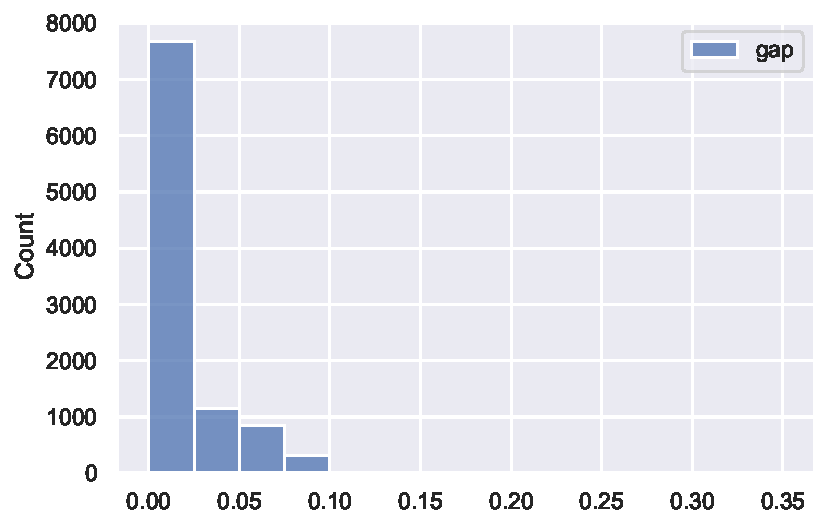
\includegraphics[width=1.2\textwidth]{figure/greedy_huffman_fig2.pdf}
    \caption{Distribution of the gap between the optimal value and the output of the Huffman-based algorithm.}
    \label{fig:greedy_huffman_2}
      \end{subfigure}
    \caption{Comparison between Huffman-based algorithm and the brute force optimal}
\end{figure}